% Options for packages loaded elsewhere
\PassOptionsToPackage{unicode}{hyperref}
\PassOptionsToPackage{hyphens}{url}
% !TeX program = pdfLaTeX
\documentclass[12pt]{article}
\usepackage{amsmath}
\usepackage{graphicx,psfrag,epsf}
\usepackage{enumerate}
\usepackage[]{natbib}
\usepackage{textcomp}


%\pdfminorversion=4
% NOTE: To produce blinded version, replace "0" with "1" below.
\newcommand{\blind}{0}

% DON'T change margins - should be 1 inch all around.
\addtolength{\oddsidemargin}{-.5in}%
\addtolength{\evensidemargin}{-1in}%
\addtolength{\textwidth}{1in}%
\addtolength{\textheight}{1.7in}%
\addtolength{\topmargin}{-1in}%

%% load any required packages here



% tightlist command for lists without linebreak
\providecommand{\tightlist}{%
  \setlength{\itemsep}{0pt}\setlength{\parskip}{0pt}}

% From pandoc table feature
\usepackage{longtable,booktabs,array}
\usepackage{calc} % for calculating minipage widths
% Correct order of tables after \paragraph or \subparagraph
\usepackage{etoolbox}
\makeatletter
\patchcmd\longtable{\par}{\if@noskipsec\mbox{}\fi\par}{}{}
\makeatother
% Allow footnotes in longtable head/foot
\IfFileExists{footnotehyper.sty}{\usepackage{footnotehyper}}{\usepackage{footnote}}
\makesavenoteenv{longtable}



\IfFileExists{bookmark.sty}{\usepackage{bookmark}}{\usepackage{hyperref}}
\IfFileExists{xurl.sty}{\usepackage{xurl}}{} % add URL line breaks if available
\hypersetup{
  pdftitle={Title here},
  pdfkeywords={3 to 6 keywords, that do not appear in the title},
  hidelinks,
  pdfcreator={LaTeX via pandoc}}



\begin{document}


\def\spacingset#1{\renewcommand{\baselinestretch}%
{#1}\small\normalsize} \spacingset{1}


%%%%%%%%%%%%%%%%%%%%%%%%%%%%%%%%%%%%%%%%%%%%%%%%%%%%%%%%%%%%%%%%%%%%%%%%%%%%%%

\if0\blind
{
  \title{\bf Title here}

  \author{
        Author 1 \thanks{The authors gratefully acknowledge \ldots{}} \\
    Department of YYY, University of XXX\\
     and \\     Author 2 \\
    Department of ZZZ, University of WWW\\
      }
  \maketitle
} \fi

\if1\blind
{
  \bigskip
  \bigskip
  \bigskip
  \begin{center}
    {\LARGE\bf Title here}
  \end{center}
  \medskip
} \fi

\bigskip
\begin{abstract}
The text of your abstract. 200 or fewer words.
\end{abstract}

\noindent%
{\it Keywords:} 3 to 6 keywords, that do not appear in the title

\vfill

\newpage
\spacingset{1.9} % DON'T change the spacing!

\hypertarget{introduction}{%
\section{Introduction}\label{introduction}}

This template demonstrates some of the basic latex you'll need to know
to create a ASA article. It is built from template find at Journal of
the American Statistical Association
\href{https://www.tandfonline.com/action/authorSubmission?show=instructions\&journalCode=uasa20\#formatting}{instruction
for authors}

\hypertarget{plot}{%
\subsection{Plot}\label{plot}}

Plot example - LaTeX floating to be adjusted if you don't want it.

\begin{figure}
\centering
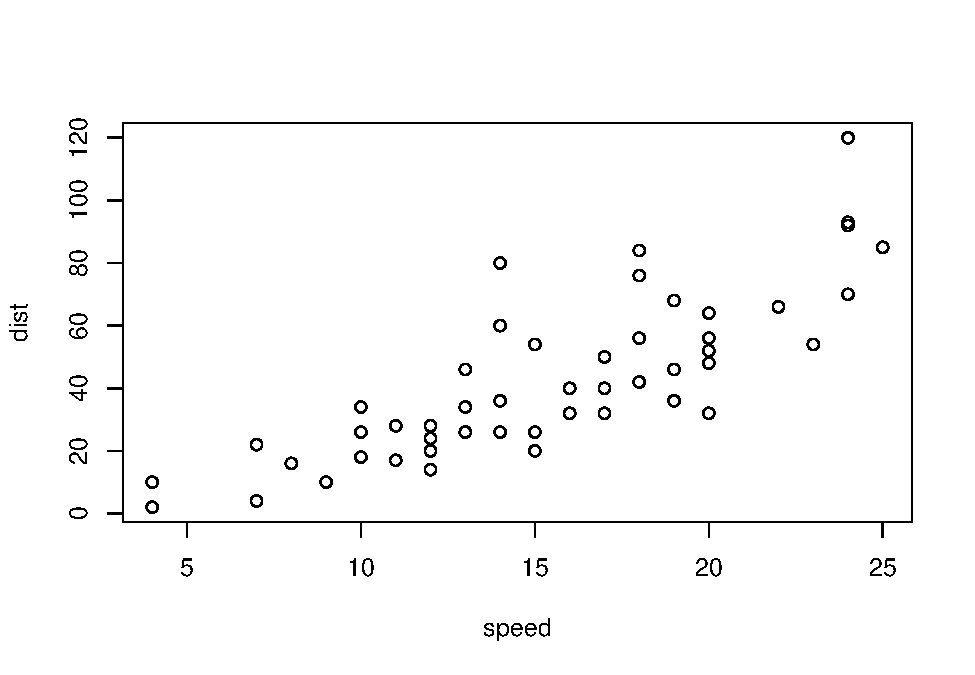
\includegraphics{try-template-2_files/figure-latex/unnamed-chunk-1-1.pdf}
\caption{A plot example}
\end{figure}

\hypertarget{table}{%
\subsection{Table}\label{table}}

Table example

\begin{longtable}[]{@{}rr@{}}
\toprule\noalign{}
speed & dist \\
\midrule\noalign{}
\endhead
\bottomrule\noalign{}
\endlastfoot
4 & 2 \\
4 & 10 \\
7 & 4 \\
7 & 22 \\
8 & 16 \\
9 & 10 \\
\end{longtable}

\hypertarget{various-guidelines}{%
\subsection{Various guidelines}\label{various-guidelines}}

\begin{itemize}
\tightlist
\item
  Note that figures and tables should appear in the paper, not at the
  end or in separate files.
\item
  Remember that in the blind version, you should not identify authors
  indirectly in the text. That is, don't say ``In Smith et. al.~(2009)
  we showed that \ldots{}''. Instead, say ``Smith et. al.~(2009) showed
  that \ldots{}''.
\item
  These points are only intended to remind you of some requirements.
  Please refer to the instructions for authors at
  \url{http://amstat.tandfonline.com/action/authorSubmission?journalCode=uasa20\&page=instructions\#.VFkk7fnF_0c}
\item
  For more about ASA~style, please see
  \url{http://journals.taylorandfrancis.com/amstat/asa-style-guide/}
\item
  If you have supplementary material (e.g., software, data, technical
  proofs), identify them in the section below. In early stages of the
  submission process, you may be unsure what to include as supplementary
  material. Don't worry---this is something that can be worked out at
  later stages.
\end{itemize}

\hypertarget{meth}{%
\section{Methods}\label{meth}}

Don't take any of these section titles seriously. They're just for
illustration.

\hypertarget{verify}{%
\section{Verifications}\label{verify}}

This section will be just long enough to illustrate what a full page of
text looks like, for margins and spacing.

\addtolength{\textheight}{.5in}%

See \citet{Campbell02} and \citet{Schubert13} or \citep{Chi81}

The quick brown fox jumped over the lazy dog. The quick brown fox jumped
over the lazy dog. The quick brown fox jumped over the lazy dog. The
quick brown fox jumped over the lazy dog. \textbf{With this spacing we
have 25 lines per page.} The quick brown fox jumped over the lazy dog.
The quick brown fox jumped over the lazy dog. The quick brown fox jumped
over the lazy dog. The quick brown fox jumped over the lazy dog. The
quick brown fox jumped over the lazy dog.

The quick brown fox jumped over the lazy dog. The quick brown fox jumped
over the lazy dog. The quick brown fox jumped over the lazy dog. The
quick brown fox jumped over the lazy dog. The quick brown fox jumped
over the lazy dog. The quick brown fox jumped over the lazy dog. The
quick brown fox jumped over the lazy dog. The quick brown fox jumped
over the lazy dog. The quick brown fox jumped over the lazy dog. The
quick brown fox jumped over the lazy dog.

The quick brown fox jumped over the lazy dog. The quick brown fox jumped
over the lazy dog. The quick brown fox jumped over the lazy dog. The
quick brown fox jumped over the lazy dog. The quick brown fox jumped
over the lazy dog. The quick brown fox jumped over the lazy dog. The
quick brown fox jumped over the lazy dog. The quick brown fox jumped
over the lazy dog. The quick brown fox jumped over the lazy dog. The
quick brown fox jumped over the lazy dog.

\addtolength{\textheight}{-.3in}%

The quick brown fox jumped over the lazy dog. The quick brown fox jumped
over the lazy dog. The quick brown fox jumped over the lazy dog. The
quick brown fox jumped over the lazy dog. The quick brown fox jumped
over the lazy dog. The quick brown fox jumped over the lazy dog. The
quick brown fox jumped over the lazy dog. The quick brown fox jumped
over the lazy dog. The quick brown fox jumped over the lazy dog. The
quick brown fox jumped over the lazy dog.

The quick brown fox jumped over the lazy dog. The quick brown fox jumped
over the lazy dog. The quick brown fox jumped over the lazy dog. The
quick brown fox jumped over the lazy dog. The quick brown fox jumped
over the lazy dog. The quick brown fox jumped over the lazy dog. The
quick brown fox jumped over the lazy dog. The quick brown fox jumped
over the lazy dog. The quick brown fox jumped over the lazy dog. The
quick brown fox jumped over the lazy dog.

The quick brown fox jumped over the lazy dog. The quick brown fox jumped
over the lazy dog. The quick brown fox jumped over the lazy dog. The
quick brown fox jumped over the lazy dog. The quick brown fox jumped
over the lazy dog. The quick brown fox jumped over the lazy dog. The
quick brown fox jumped over the lazy dog. The quick brown fox jumped
over the lazy dog. The quick brown fox jumped over the lazy dog. The
quick brown fox jumped over the lazy dog.

The quick brown fox jumped over the lazy dog. The quick brown fox jumped
over the lazy dog. The quick brown fox jumped over the lazy dog. The
quick brown fox jumped over the lazy dog. The quick brown fox jumped
over the lazy dog. The quick brown fox jumped over the lazy dog. The
quick brown fox jumped over the lazy dog. The quick brown fox jumped
over the lazy dog. The quick brown fox jumped over the lazy dog. The
quick brown fox jumped over the lazy dog.

The quick brown fox jumped over the lazy dog. The quick brown fox jumped
over the lazy dog. The quick brown fox jumped over the lazy dog. The
quick brown fox jumped over the lazy dog. The quick brown fox jumped
over the lazy dog. The quick brown fox jumped over the lazy dog. The
quick brown fox jumped over the lazy dog. The quick brown fox jumped
over the lazy dog. The quick brown fox jumped over the lazy dog. The
quick brown fox jumped over the lazy dog.

The quick brown fox jumped over the lazy dog. The quick brown fox jumped
over the lazy dog. The quick brown fox jumped over the lazy dog. The
quick brown fox jumped over the lazy dog. The quick brown fox jumped
over the lazy dog. The quick brown fox jumped over the lazy dog. The
quick brown fox jumped over the lazy dog. The quick brown fox jumped
over the lazy dog. The quick brown fox jumped over the lazy dog. The
quick brown fox jumped over the lazy dog.

The quick brown fox jumped over the lazy dog. The quick brown fox jumped
over the lazy dog. The quick brown fox jumped over the lazy dog. The
quick brown fox jumped over the lazy dog. The quick brown fox jumped
over the lazy dog. The quick brown fox jumped over the lazy dog. The
quick brown fox jumped over the lazy dog. The quick brown fox jumped
over the lazy dog. The quick brown fox jumped over the lazy dog. The
quick brown fox jumped over the lazy dog.

The quick brown fox jumped over the lazy dog. The quick brown fox jumped
over the lazy dog. The quick brown fox jumped over the lazy dog. The
quick brown fox jumped over the lazy dog.

\hypertarget{conc}{%
\section{Conclusion}\label{conc}}

\bigskip

\begin{center}
\textbf{SUPPLEMENTARY MATERIAL}

\end{center}

\begin{quote}
Use \href{https://pandoc.org/MANUAL.html\#definition-lists}{definition
list syntax} in this part
\end{quote}

\begin{description}
\tightlist
\item[Title:]
Brief description. (file type)
\item[R-package for MYNEW routine:]
R-package \textbf{MYNEW} containing code to perform the diagnostic
methods described in the article. The package also contains all datasets
used as examples in the article. (GNU zipped tar file)
\item[HIV data set:]
Data set used in the illustration of MYNEW method in
Section\textasciitilde{} 3.2. (.txt file)
\end{description}

\hypertarget{bibliography.}{%
\section{Bibliography.}\label{bibliography.}}

Using \texttt{natbib} is the default with this format, using
\texttt{plain.bst} by default on the template, and \texttt{apalike.bst}
in this Rmd skeleton. Chante to your preference using the
\texttt{biblio-style} in YAML

\bibliographystyle{apalike}
\bibliography{bibliography.bib}



\end{document}
